\documentclass[10pt,twoside]{ctexart}
\usepackage[utf8]{inputenc}
\usepackage[T1]{fontenc}
\usepackage{url}
\usepackage{xeCJK}
\usepackage{xeCJKfntef}
\usepackage{listings}
\usepackage{color}
\usepackage{xcolor}
\usepackage{subfigure}
\usepackage{titletoc}
\usepackage{wrapfig}
\usepackage{bm}
\usepackage{fancyhdr}
\usepackage{indentfirst}  
\usepackage{amsmath}
\usepackage{amsfonts}
\usepackage{fancybox}
\usepackage{amssymb}
\usepackage{graphicx}
\usepackage{paracol}
\usepackage{bbm}
\usepackage{bbold}
\usepackage{verbatim}
\usepackage{CJKulem}
\usepackage{ulem}
\usepackage{soul}
\usepackage{tikz}
\usepackage{lastpage} %总页数
\usepackage[left=2cm, right=2cm, top=1.5cm, bottom=1.5cm,a4paper]{geometry}
%%%%%%%%%%%%%%%%%%%%%%%%%%%%%%%%%%%%%%%%%%%%%%%%%%%%%%%%%%%%%%%%%%%%%%%%%%%%%%%%
%																			   %
%																			   %
%																			   %
%																			   %
%																			   %
%																			   %
%---------------------------设置                							    %
%																			   %
%																			   %
%																			   %
%																			   %
%																			   %
%																			   %
%%%%%%%%%%%%%%%%%%%%%%%%%%%%%%%%%%%%%%%%%%%%%%%%%%%%%%%%%%%%%%%%%%%%%%%%%%%%%%%%
\setCJKmainfont{STLibianSC-Regular}
%
\setmainfont{Times New Roman}

%\CTEXsetup[format={\Large\bfseries}]{section}	% 标题右对齐
\pagestyle{fancy}
\thispagestyle{empty}	% 去除页眉

\setlength{\parindent}{2em}% 缩进
\setlength{\parskip}{1ex} % 段间距
\definecolor{dkgreen}{rgb}{0,0.6,0}
\definecolor{gray}{rgb}{0.5,0.5,0.5}
\definecolor{mauve}{rgb}{0.58,0,0.82}
\definecolor{tigray}{rgb}{0.96,0.96,0.96}
\lstset{
	%backgroundcolor=\color[RGB]{245,245,244},
	basicstyle=\tt,
    keywordstyle=\color{purple}\bfseries,
    identifierstyle=\color{brown!80!black},
    commentstyle=\color{gray},
	frameround=fttt,
	frame=trBL,
	language=c,
	aboveskip=3mm,
	belowskip=3mm,
	showstringspaces=false,
	columns=fixed,
	%basicstyle={\small},
	numbers=none,%设置行号位置none不显示行号
	%numberstyle=\tiny\courier, %设置行号大小
	numberstyle=\tiny\color{gray},
	%keywordstyle=\color{red},
	%commentstyle=\color{dkgreen},
	stringstyle=\color{mauve},
	breaklines=ture,
	breakatwhitespace=false,
	escapeinside=``,%逃逸字符(1左面的键),用于显示中文例如在代码中`中文...`
	tabsize=4,
	extendedchars=false %解决代码跨页时,章节标题,页眉等汉字不显示的问题
}


\begin{document}
\footnotelayout{m}
\newcommand*{\subsectionname}{{\tt 1.1}基础}
\fancyhead[RE]{\subsectionname}
\fancyhead[OL]{\leftmark}
\fancyhead[LE,RO]{\tt PAGE \thepage\space of\space \pageref{LastPage}}

\renewcommand{\footrulewidth}{0.5pt}
\fancyfoot[CE,CO]{\tt OBTUSE}


\begin{titlepage}
	\begin{center}
	  	\quad
  
	  	\vspace{.2\textheight}
	 	\huge\textbf{\tt Obtuse}
		
		\vspace{2ex}

	 	
		\vspace{2ex}
	  	\normalsize {\tt Wenqingqian}
  
 
	\end{center}
\end{titlepage}

\newpage
\thispagestyle{empty}
\begin{titlepage}
	\begin{center}
		\quad

		\vspace{.2\textheight}
		\tikzset{every picture/.style={line width=0.75pt}} %set default line width to 0.75pt        

		\begin{tikzpicture}[x=0.75pt,y=0.75pt,yscale=-1,xscale=1]
		%uncomment if require: \path (0,522); %set diagram left start at 0, and has height of 522
		
		%Shape: Arc [id:dp3943727375387953] 
		\draw  [draw opacity=0] (332.95,517) .. controls (332.47,517) and (331.98,517) .. (331.5,517) .. controls (192.05,517) and (79,410.44) .. (79,279) .. controls (79,147.56) and (192.05,41) .. (331.5,41) .. controls (331.68,41) and (331.86,41) .. (332.04,41) -- (331.5,279) -- cycle ; \draw   (332.95,517) .. controls (332.47,517) and (331.98,517) .. (331.5,517) .. controls (192.05,517) and (79,410.44) .. (79,279) .. controls (79,147.56) and (192.05,41) .. (331.5,41) .. controls (331.68,41) and (331.86,41) .. (332.04,41) ;  
		%Curve Lines [id:da4428105762057488] 
		\draw    (332.04,41) .. controls (513,247) and (109,278) .. (332.95,517) ;
		%Shape: Circle [id:dp5261183402750851] 
		\draw   (209,147.5) .. controls (209,140.04) and (215.04,134) .. (222.5,134) .. controls (229.96,134) and (236,140.04) .. (236,147.5) .. controls (236,154.96) and (229.96,161) .. (222.5,161) .. controls (215.04,161) and (209,154.96) .. (209,147.5) -- cycle ;
		%Shape: Circle [id:dp5452006509569032] 
		\draw   (406,376.5) .. controls (406,369.04) and (412.04,363) .. (419.5,363) .. controls (426.96,363) and (433,369.04) .. (433,376.5) .. controls (433,383.96) and (426.96,390) .. (419.5,390) .. controls (412.04,390) and (406,383.96) .. (406,376.5) -- cycle ;	
		\end{tikzpicture}		
	\end{center}
	\begin{center}
	 	\normalsize %test on gcc 12.2.0
		
	 	%\vspace{2ex}
	  	%\normalsize 所有实验均使用 gcc 12.2.0 编译器

	  	\vfill
	  	{\tt wenqq3@outlook.com}

		%\vspace{2ex}
		%\normalsize Dont pay for what u dont use
	\end{center}
\end{titlepage}

\newpage
\thispagestyle{empty}
\tableofcontents
\shadowsize=0.5mm
\newpage
\setcounter{page}{1}
%%%%%%%%%%%%%%%%%%%%%%%%%%%%%%%%%%%%%%%%%%%%%%%%%%%%%%%%%%%%%%%%%%%%%%%%%%%%%%%%
%																			   %
%																			   %
%																			   %
%																			   %
%																			   %
%																			   %
%---------------------------C++                 							   %
%																			   %
%																			   %
%																			   %
%																			   %
%																			   %
%																			   %
%%%%%%%%%%%%%%%%%%%%%%%%%%%%%%%%%%%%%%%%%%%%%%%%%%%%%%%%%%%%%%%%%%%%%%%%%%%%%%%%
\section{\tt C++}
\subsection{基础}
\subsubsection[ISOK:{\tt C}和{\tt C++}区别]{\color{purple}{{\tt C}和{\tt C++}区别}}
\begin{itemize}
	\item {\tt C}语言是{\tt C++}的子集, {\tt C++}可以很好兼容{\tt C}语言. 但是{\tt C++}又有很多新特性, 如引用、智能指针、{\tt auto}变量等
	\item {\tt C++}是面对对象的编程语言; {\tt C}语言是面对过程的编程语言
	\item {\tt C}语言有一些不安全的语言特性, 如指针使用的潜在危险、强制转换的不确定性、内存泄露等. 而{\tt C++}对此增加了不少新特性来改善安全性, 如{\tt const}常量、引用、{\tt cast}转换、智能指针、{\tt try—catch}等等
	\item {\tt C++}可复用性高, {\tt C++}引入了模板的概念, 后面在此基础上, 实现了方便开发的标准模板库{\tt STL}. {\tt C++}的{\tt STL}库相对于{\tt C}语言的函数库更灵活、更通用
\end{itemize}
\subsubsection[多态的实现原理和应用场景]{\color{purple}{多态的实现原理和应用场景}}
\subsubsection[线程安全的实现及标准容器库的线程安全性]{\color{purple}{线程安全的实现及标准容器库的线程安全性}}
\subsubsection[{\tt sort}算法是怎么实现的]{\color{purple}{{\tt sort}算法是怎么实现的}}
\subsubsection[{\tt malloc}和{\tt new}区别]{\color{purple}{{\tt malloc}和{\tt new}区别}}
\subsubsection[ISOK:{\tt C++}从代码到可执行二进制文件的过程]{\color{purple}{{\tt C++}从代码到可执行二进制文件的过程}}
\begin{enumerate}
	\item 预编译: 这个过程主要的处理操作如下
	\begin{enumerate}
		\item 将所有的{\tt \#define}删除, 并且展开所有的宏定义
		\item 处理所有的条件预编译指令, 如{\tt \#if、\#ifdef}
		\item 处理{\tt \#include}预编译指令, 将被包含的文件插入到该预编译指令的位置
		\item 过滤所有的注释
		\item 添加行号和文件名标识
	\end{enumerate}
	\item 编译: 这个过程主要的处理操作如下
	\begin{enumerate}
		\item 词法分析: 将源代码的字符序列分割成一系列的记号
		\item 语法分析: 对记号进行语法分析, 产生语法树
		\item 语义分析: 判断表达式是否有意义
		\item 代码优化
		\item 目标代码生成: 生成汇编代码
		\item 目标代码优化
	\end{enumerate}
	\item 汇编: 这个过程主要是将汇编代码转变成机器可以执行的指令
	\item 将不同的源文件产生的目标文件进行链接, 从而形成一个可以执行的程序
	\begin{itemize}
		\item 链接分为静态链接和动态链接
		\item 静态链接, 是在链接的时候就已经把要调用的函数或者过程链接到了生成的可执行文件中, 
				就算你在去把静态库删除也不会影响可执行程序的执行; 生成的静态链接库, {\tt Windows}下以{\tt .lib}为后缀, 
				{\tt Linux}下以{\tt .a}为后缀
		\item 而动态链接, 是在链接的时候没有把调用的函数代码链接进去, 而是在执行的过程中, 再去找要链接的函数, 
				生成的可执行文件中没有函数代码, 只包含函数的重定位信息, 所以当你删除动态库时, 可执行程序就不能运行
				生成的动态链接库, {\tt Windows}下以{\tt .dll}为后缀, {\tt Linux}下以{\tt .so}为后缀
	\end{itemize}
\end{enumerate}
\subsubsection[ISOK:{\tt static}关键字]{\color{purple}{{\tt static}关键字}}
\begin{enumerate}
	\item 全局静态变量和局部静态变量: 初始化的静态变量会在数据段分配内存, 未初始化的静态变量会在{\tt BSS}段分配内存. 
			直到程序结束, 静态变量始终会维持前值. 只不过全局静态变量和局部静态变量的作用域不一样
	\item 静态函数: 静态函数只能在本源文件(该翻译单元)中使用
	\item 类中的静态成员变量: 静态数据成员, 隐藏在类作用域中的全局变量(可以通过类名({\tt Class::})或类对象访问). 
			类中的{\tt static}静态数据成员拥有一块单独的存储区, 而不管创建了多少个该类的对象. 
			所有这些对象的静态数据成员都共享这一块静态存储空间
	\item 类中的静态成员函数: 静态成员函数也是类的一部分, 而不是对象的一部分
		\\  只能访问静态数据成员: 
			当调用一个对象的非静态成员函数时, 系统会把该对象的起始地址赋给成员函数的this指针. 
			而静态成员函数不属于任何一个对象, 因此{\tt C++}规定\uline{静态成员函数没有{\tt this}指针}. 
			既然它没有指向某一对象, 也就无法对一个对象中的非静态成员进行访问
\end{enumerate}

\subsubsection[ISOK:{\tt extern}关键字与链接性]{\color{purple}{{\tt extern}关键字与链接性}}

在{\tt C++}中, 翻译单元由实现文件及直接或间接包含的所有标头组成

\begin{center}
\tikzset{every picture/.style={line width=0.75pt}} %set default line width to 0.75pt        

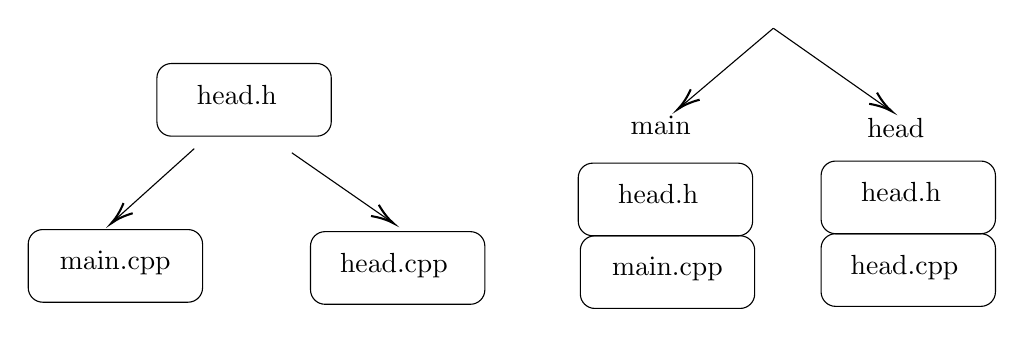
\begin{tikzpicture}[x=0.75pt,y=0.75pt,yscale=-1,xscale=1]
%uncomment if require: \path (0,300); %set diagram left start at 0, and has height of 300

%Rounded Rect [id:dp8046212658933671] 
\draw   (119,83) .. controls (119,79.13) and (122.13,76) .. (126,76) -- (196,76) .. controls (199.87,76) and (203,79.13) .. (203,83) -- (203,104) .. controls (203,107.87) and (199.87,111) .. (196,111) -- (126,111) .. controls (122.13,111) and (119,107.87) .. (119,104) -- cycle ;
%Rounded Rect [id:dp4131717476038639] 
\draw   (57,163) .. controls (57,159.13) and (60.13,156) .. (64,156) -- (134,156) .. controls (137.87,156) and (141,159.13) .. (141,163) -- (141,184) .. controls (141,187.87) and (137.87,191) .. (134,191) -- (64,191) .. controls (60.13,191) and (57,187.87) .. (57,184) -- cycle ;
%Rounded Rect [id:dp6275602235598181] 
\draw   (193,164) .. controls (193,160.13) and (196.13,157) .. (200,157) -- (270,157) .. controls (273.87,157) and (277,160.13) .. (277,164) -- (277,185) .. controls (277,188.87) and (273.87,192) .. (270,192) -- (200,192) .. controls (196.13,192) and (193,188.87) .. (193,185) -- cycle ;
%Straight Lines [id:da29892507643017163] 
\draw    (137,117) -- (98.49,151.66) ;
\draw [shift={(97,153)}, rotate = 318.01] [color={rgb, 255:red, 0; green, 0; blue, 0 }  ][line width=0.75]    (10.93,-3.29) .. controls (6.95,-1.4) and (3.31,-0.3) .. (0,0) .. controls (3.31,0.3) and (6.95,1.4) .. (10.93,3.29)   ;
%Straight Lines [id:da7604434249637251] 
\draw    (184,119) -- (231.36,151.86) ;
\draw [shift={(233,153)}, rotate = 214.76] [color={rgb, 255:red, 0; green, 0; blue, 0 }  ][line width=0.75]    (10.93,-3.29) .. controls (6.95,-1.4) and (3.31,-0.3) .. (0,0) .. controls (3.31,0.3) and (6.95,1.4) .. (10.93,3.29)   ;
%Rounded Rect [id:dp8118464469584348] 
\draw   (439,165) .. controls (439,161.13) and (442.13,158) .. (446,158) -- (516,158) .. controls (519.87,158) and (523,161.13) .. (523,165) -- (523,186) .. controls (523,189.87) and (519.87,193) .. (516,193) -- (446,193) .. controls (442.13,193) and (439,189.87) .. (439,186) -- cycle ;
%Rounded Rect [id:dp6893102005714937] 
\draw   (323,166) .. controls (323,162.13) and (326.13,159) .. (330,159) -- (400,159) .. controls (403.87,159) and (407,162.13) .. (407,166) -- (407,187) .. controls (407,190.87) and (403.87,194) .. (400,194) -- (330,194) .. controls (326.13,194) and (323,190.87) .. (323,187) -- cycle ;
%Rounded Rect [id:dp2970948370150095] 
\draw   (322,131) .. controls (322,127.13) and (325.13,124) .. (329,124) -- (399,124) .. controls (402.87,124) and (406,127.13) .. (406,131) -- (406,152) .. controls (406,155.87) and (402.87,159) .. (399,159) -- (329,159) .. controls (325.13,159) and (322,155.87) .. (322,152) -- cycle ;
%Rounded Rect [id:dp3048285006841027] 
\draw   (439,130) .. controls (439,126.13) and (442.13,123) .. (446,123) -- (516,123) .. controls (519.87,123) and (523,126.13) .. (523,130) -- (523,151) .. controls (523,154.87) and (519.87,158) .. (516,158) -- (446,158) .. controls (442.13,158) and (439,154.87) .. (439,151) -- cycle ;
%Straight Lines [id:da8496668043021236] 
\draw    (416,59) -- (371.53,96.71) ;
\draw [shift={(370,98)}, rotate = 319.71] [color={rgb, 255:red, 0; green, 0; blue, 0 }  ][line width=0.75]    (10.93,-3.29) .. controls (6.95,-1.4) and (3.31,-0.3) .. (0,0) .. controls (3.31,0.3) and (6.95,1.4) .. (10.93,3.29)   ;
%Straight Lines [id:da057864555520047656] 
\draw    (416,59) -- (471.36,97.85) ;
\draw [shift={(473,99)}, rotate = 215.06] [color={rgb, 255:red, 0; green, 0; blue, 0 }  ][line width=0.75]    (10.93,-3.29) .. controls (6.95,-1.4) and (3.31,-0.3) .. (0,0) .. controls (3.31,0.3) and (6.95,1.4) .. (10.93,3.29)   ;

% Text Node
\draw (137,85) node [anchor=north west][inner sep=0.75pt]   [align=left] {head.h};
% Text Node
\draw (71,165) node [anchor=north west][inner sep=0.75pt]   [align=left] {main.cpp};
% Text Node
\draw (206,166) node [anchor=north west][inner sep=0.75pt]   [align=left] {head.cpp};
% Text Node
\draw (452,167) node [anchor=north west][inner sep=0.75pt]   [align=left] {head.cpp};
% Text Node
\draw (337,168) node [anchor=north west][inner sep=0.75pt]   [align=left] {main.cpp};
% Text Node
\draw (340,133) node [anchor=north west][inner sep=0.75pt]   [align=left] {head.h};
% Text Node
\draw (457,132) node [anchor=north west][inner sep=0.75pt]   [align=left] {head.h};
% Text Node
\draw (346,100) node [anchor=north west][inner sep=0.75pt]   [align=left] {main};
% Text Node
\draw (460,101) node [anchor=north west][inner sep=0.75pt]   [align=left] {head};


\end{tikzpicture}
\end{center}

\noindent 每个翻译单元由编译器单独编译, 最终将得到的.o文件链接得到可执行文件. 如上图所示程序结构, 在链接时会出现如下问题:

假如在{\tt head.h}文件中定义一个外部链接性变量.
\begin{lstlisting}
#ifndef HEAD_H
#define HEAD_H
int i = 0;
#endif
\end{lstlisting}
那么在链接时就会出错, 原因是如上两个翻译单元相当于

\begin{center}
\tikzset{every picture/.style={line width=0.75pt}} %set default line width to 0.75pt        

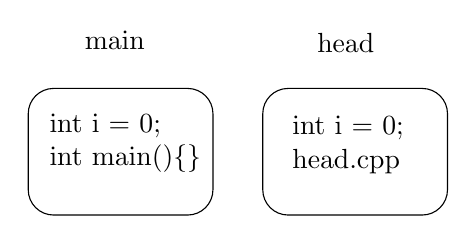
\begin{tikzpicture}[x=0.75pt,y=0.75pt,yscale=-1,xscale=1]
%uncomment if require: \path (0,300); %set diagram left start at 0, and has height of 300

%Rounded Rect [id:dp31960853174211556] 
\draw   (225,159.2) .. controls (225,152.46) and (230.46,147) .. (237.2,147) -- (301.8,147) .. controls (308.54,147) and (314,152.46) .. (314,159.2) -- (314,195.8) .. controls (314,202.54) and (308.54,208) .. (301.8,208) -- (237.2,208) .. controls (230.46,208) and (225,202.54) .. (225,195.8) -- cycle ;
%Rounded Rect [id:dp47295061263468985] 
\draw   (338,159.2) .. controls (338,152.46) and (343.46,147) .. (350.2,147) -- (414.8,147) .. controls (421.54,147) and (427,152.46) .. (427,159.2) -- (427,195.8) .. controls (427,202.54) and (421.54,208) .. (414.8,208) -- (350.2,208) .. controls (343.46,208) and (338,202.54) .. (338,195.8) -- cycle ;

% Text Node
\draw (251,118) node [anchor=north west][inner sep=0.75pt]   [align=left] {main};
% Text Node
\draw (363,119) node [anchor=north west][inner sep=0.75pt]   [align=left] {head};
% Text Node
\draw (234,158) node [anchor=north west][inner sep=0.75pt]   [align=left] {int i = 0;\\int main()\{\}};
% Text Node
\draw (351,159.2) node [anchor=north west][inner sep=0.75pt]   [align=left] {int i = 0;\\head.cpp};


\end{tikzpicture}
\end{center}
在两个文件中都定义了具有外部链接性的变量i.

在一个作用域内, 变量能且只能被定义一次, 但是可以被多次声明({\tt one define rule})
\begin{paracol}{2}
	\begin{leftcolumn}
		\begin{lstlisting}[title=定义,xleftmargin=2em,xrightmargin=2em]
// 不能在局部作用域内使用
extern int v = 0; 
int v;
		\end{lstlisting}
	\end{leftcolumn}
	\begin{rightcolumn}
		\begin{lstlisting}[title=声明,xleftmargin=2em,xrightmargin=2em]
void func();
extern void func();
extern int v;
		\end{lstlisting}
	\end{rightcolumn}
\end{paracol}

如果需要在多个文件, 指个多翻译单元中使用同一变量, 就必须把定义与声明分离. 变量的定义只能出现在一个文件中, 而在其它用到该变量
	的文件中对其声明.

所以往往头文件中只放一些声明而在另外的文件中进行定义.

\begin{paracol}{2}
	\begin{leftcolumn}
		常见的内部链接类型
		\begin{enumerate}
			\item {\tt const}全局变量
			\item {\tt static}全局变量
			\item {\tt static}函数
			\item {\tt inline}\footnote[1]{{\tt inline} 现在表示在链接时遇到不同编译单元出现了相同签名的函数时只保留一份, 不在是內联的意思.}函数/变量\footnote[2]{{\tt inline variable is C++17 extension}}
			\item 类内定义的成员函数
			\item 类内定义的数据成员(即非静态数据成员)
		\end{enumerate}
	\end{leftcolumn}
	\begin{rightcolumn}
		常见的外部链接类型
		\begin{enumerate}
			\item 全局变量与函数(非{\tt const、static、inline})
			\item 类外定义的数据成员(即静态数据成员在类外的定义)
			\item 类外定义的成员函数
			\item {\tt extern const T v = INIT;}
		\end{enumerate}
	\end{rightcolumn}
\end{paracol}
其它可视为无链接

\vspace{1em}
所有文件中的外部链接性变量会传递给链接器得到一张导出符号表. 记录本编译单元定义, 并且可提供给其它单元
	使用的符号及在本单元对应的地址. 

所有文件中的声明会传递给链接器得到一张未解决符号表, 记录本编译单元有声明但不在本单元定义的符号及其对应的地址, 
	显然在导出符号表中不能存在相同的符号.

{\tt C11}标准关于{\tt static}和{\tt extern}的内容:
\begin{enumerate}
	\item 若在{\tt extern}声明标识符之前的可见范围内存在对该标识符的声明, 则该标识符的链接与先前声明相同. 
			若无先前声明, 或声明无链接, 则该标识符具有外部链接
	\item 如果在同一翻译单元内, 同一标识符同时出现内外部链接, 则行为未定义
\end{enumerate}
上述原文:

{\tt For an identifier declared with the storage-class specifier extern in a scope 
in which a prior declaration of that identifier is visible, if the prior 
declaration specifies internal or external linkage, the linkage of the 
identifier at the later declaration is the same as the linkage specified 
at the prior declaration. If no prior declaration is visible, or if the 
prior declaration specifies no linkage, then the identifier has external 
linkage.

If, within a translation unit, the same identifier appears with both internal 
and external linkage, the behavior is undefined.}
%%%%%%%%%%%%%%%%%%%%%%%%%%%%%%%%%%%%%%%%%%%%%%%%%%%%%%%%%%%%%%%%%%%%%%%%%%%%%%%%
%																			   %
%																			   %
%																			   %
%																			   %
%																			   %
%																			   %
%---------------------------OS                  							   %
%																			   %
%																			   %
%																			   %
%																			   %
%																			   %
%																			   %
%%%%%%%%%%%%%%%%%%%%%%%%%%%%%%%%%%%%%%%%%%%%%%%%%%%%%%%%%%%%%%%%%%%%%%%%%%%%%%%%
\newpage
\section{\tt Operating\space System}
\subsection[\tt Linux]{\color{blue}{\tt Linux}}
\subsubsection[{\tt Linux}常见命令]{\color{purple}{{\tt Linux}常见命令}}


%%%%%%%%%%%%%%%%%%%%%%%%%%%%%%%%%%%%%%%%%%%%%%%%%%%%%%%%%%%%%%%%%%%%%%%%%%%%%%%%
%																			   %
%																			   %
%																			   %
%																			   %
%																			   %
%																			   %
%---------------------------CN                							       %
%																			   %
%																			   %
%																			   %
%																			   %
%																			   %
%																			   %
%%%%%%%%%%%%%%%%%%%%%%%%%%%%%%%%%%%%%%%%%%%%%%%%%%%%%%%%%%%%%%%%%%%%%%%%%%%%%%%%
\newpage
\section{\tt Computer\space Networking}


\subsection[\tt TCP/IP]{\color{blue}{\tt TCP/IP}}%-----------------TCP/IP-------------------
\subsubsection[{\tt TCP/IP}协议中的三次握手和四次挥手]{\color{purple}{{\tt TCP/IP}协议中的三次握手和四次挥手}}


%%%%%%%%%%%%%%%%%%%%%%%%%%%%%%%%%%%%%%%%%%%%%%%%%%%%%%%%%%%%%%%%%%%%%%%%%%%%%%%%
%																			   %
%																			   %
%																			   %
%																			   %
%																			   %
%																			   %
%---------------------------Socket                							   %
%																			   %
%																			   %
%																			   %
%																			   %
%																			   %
%																			   %
%%%%%%%%%%%%%%%%%%%%%%%%%%%%%%%%%%%%%%%%%%%%%%%%%%%%%%%%%%%%%%%%%%%%%%%%%%%%%%%%
\newpage
\section{\tt Socket}
\subsection[{\tt IO}多路复用]{\color{blue}{{\tt IO}多路复用}}


%%%%%%%%%%%%%%%%%%%%%%%%%%%%%%%%%%%%%%%%%%%%%%%%%%%%%%%%%%%%%%%%%%%%%%%%%%%%%%%%
%																			   %
%																			   %
%																			   %
%																			   %
%																			   %
%																			   %
%---------------------------DS                							       %
%																			   %
%																			   %
%																			   %
%																			   %
%																			   %
%																			   %
%%%%%%%%%%%%%%%%%%%%%%%%%%%%%%%%%%%%%%%%%%%%%%%%%%%%%%%%%%%%%%%%%%%%%%%%%%%%%%%%
\newpage
\section{\tt Data\space Structure}


%%%%%%%%%%%%%%%%%%%%%%%%%%%%%%%%%%%%%%%%%%%%%%%%%%%%%%%%%%%%%%%%%%%%%%%%%%%%%%%%
%																			   %
%																			   %
%																			   %
%																			   %
%																			   %
%																			   %
%---------------------------DB                							       %
%																			   %
%																			   %
%																			   %
%																			   %
%																			   %
%																			   %
%%%%%%%%%%%%%%%%%%%%%%%%%%%%%%%%%%%%%%%%%%%%%%%%%%%%%%%%%%%%%%%%%%%%%%%%%%%%%%%%
\newpage
\section{\tt Database}


\end{document}